\newpage
\section{Durchführung}
\subsection{Justierung}
Zunächst werden die beiden Schwingkreise auf die gleiche Resonanzfrequenz eingestellt.
Die Größenordung ermittelt man dabei, indem das Strommaximum des linken Schwingkreises sucht.
Die dazu gehörige Frequent sntspricht dabei in etwa der Resonanzfrequent.\\
Für eine genauere Ermittlung untersuche man mit Hilfe der Lissajous-Figure die Phase $\varphi$
zwischen der Generatorspannung und dem Schwingkreisstrom. Im Falle der Resonanz ist $\varphi=0$.
Nun wird der zweite Schwinkreis mithilfe einer regelbaren Kapazität auf diese Resonanzfrequenz
abgestimmt.\newline

Für einen groben Frequenzbereich für einen beobachtbaren Energieaustausch gilt 
mit $L=32$mH und $C=0.8nF$
\begin{equation}
    \omega = \frac{1}{2 \pi \sqrt{L\cdot C}} = \frac{1}{2 \pi \sqrt{32\cdot 10^{-3}\cdot 0.8\cdot 10^{-9}}}\approx 31.5\text{kHz} 
\end{equation}   
\begin{figure}
    \centering
    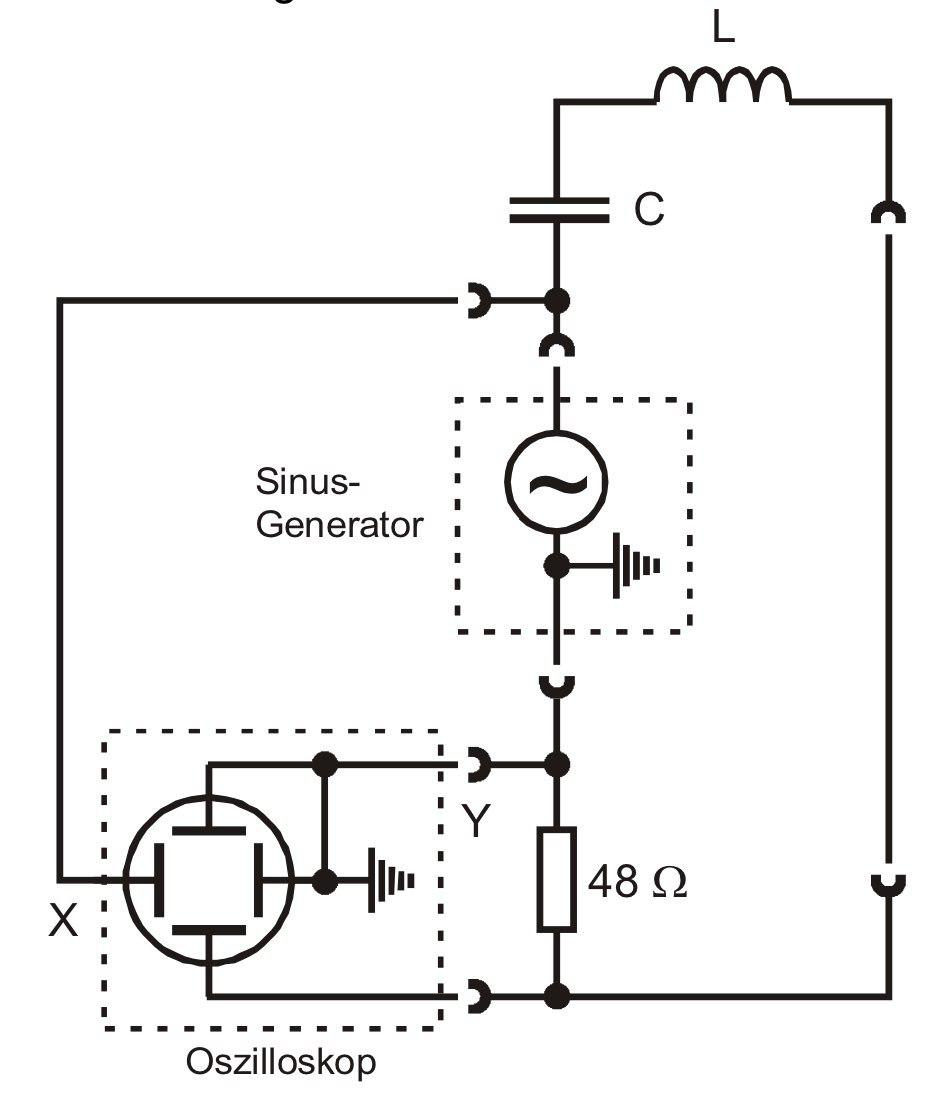
\includegraphics[width=0.4\textwidth]{bilder/justierung.jpg}
    \caption{
        Schaltung zur genauen Bestimmtung der Resonanzfrequenz.
        Dabei wird ein Schwingkreis an einen Sinusgenerator angeschlossen.
        Jeweils der Strom des Generators und des Schwingkreises werden auf 
        dem Oszilliskop im XY-Betrieb betrachtet. \cite[305]{Anleitung}
    }
    \label{fig:justierung}
\end{figure}


\subsection{Austausch der Schwingungsenergie zwischen den Einzelsystemen}
Mit einer Rechteckspannung wird einer der Schwinkreise angeregt während der andere
keine externe erregung ausgesetzt wird. Die beiden Schwingkreise sind dabei über den
Kopplungskondensator $C_k$ gekoppelt. Die Schwingungsenergie kann mithilfe des
Oszilliskop am Kopplungsglied betrachtet werden.\\
Die entstehende Schwebung der Form \ref{schw1} und \ref{schw2}
wird am Oszilliskop beobachtet.\\
Somit kann ein Verhältnis zwischen der Schwingungs- und Schwebungsfrequenz in 
Abhängigkeit der Größe des Koppelkondensator $C_k$ mit $2\leq C_k \leq 12$nF ermittelt 
werden, durch die Anzahl der Schwingsmaxima innerhal einer Schwebungperiode.
\begin{figure}
    \centering
    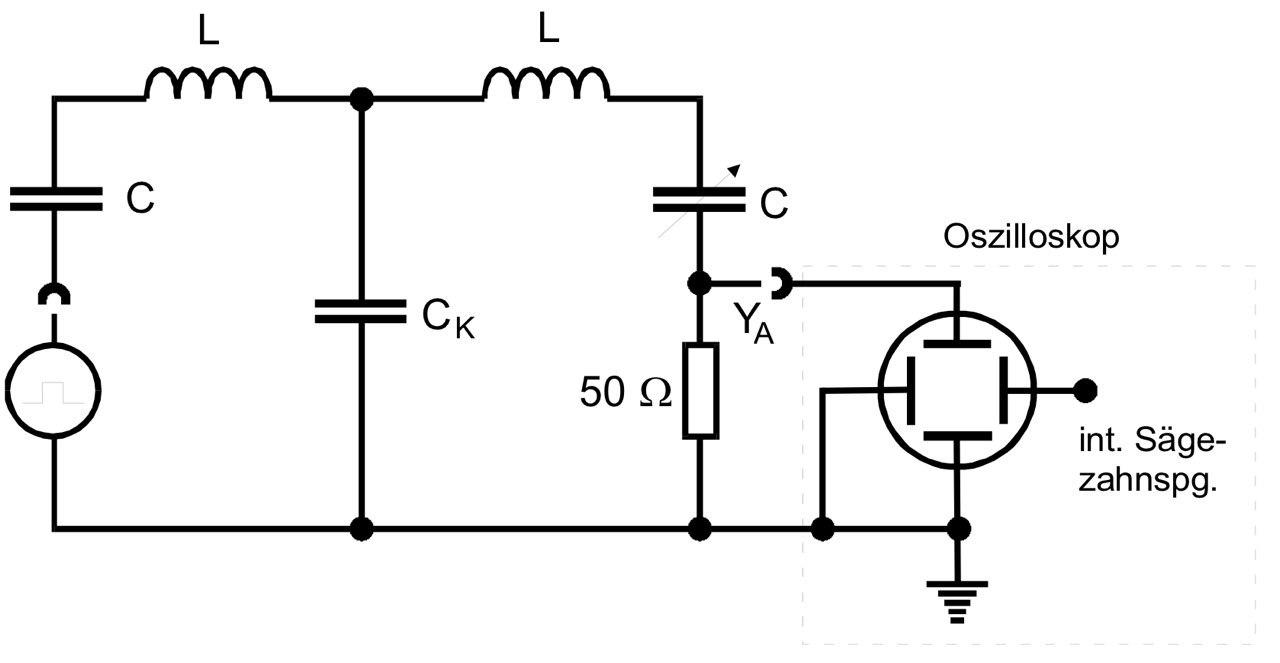
\includegraphics[width=0.5\textwidth]{bilder/a.jpg}
    \caption{
        Schaltbild zur Untersucheng der Energieübertragung zwischen den Einzelsystemen
        durch Schwebungsvorgänge. \cite[306]{Anleitung}
    }
    \label{fig:Versuchsaufbau}
\end{figure}
\subsection{Fundermentalschwingungen}
Die rechtecksignal aus Abbildung \ref{fig:Versuchsaufbau} wird durch ein Sinussignal
ersetzt. Mit den Lissajous-Figuren bei denen die X-Komponente die Generatorspannung 
und die Y Komponente den Schwingkreis wiederspieglet.
Man findet die Fundermentalschwingungen in Abhängigkeit von $C_k$ bei $\varphi=0$ bzw $\varphi=\frac{\pi}{2}$.\\

\subsection{Verlauf der Ströme}
Nun betrachte man den Verlauf der Ströme $I_2$ und $I_k$ in Abhängigkeit der Frequenz.






\label{sec:Durchfuehrung}
